\begin{figure}[h]
\centering
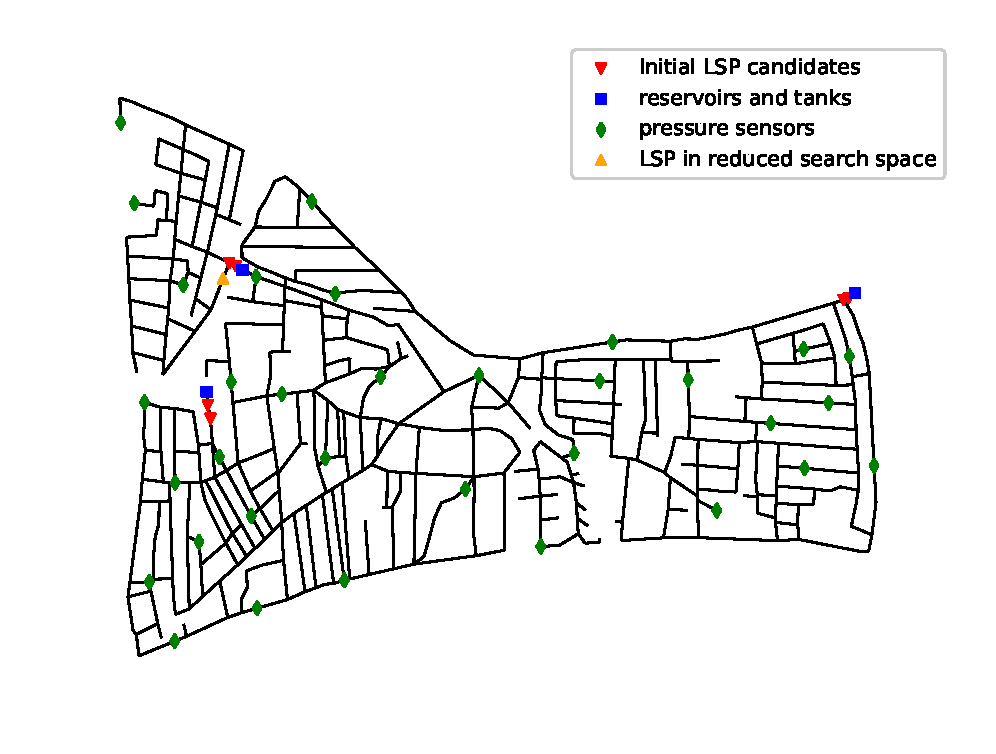
\includegraphics[height=0.3\textheight,width=\textwidth,keepaspectratio=True]{Figures/lsp_candidates_ltown.eps}
\caption{Analysis of the L-Town network with Bisection Search for fixed
starting times. Points with a low detector sensitivity are located
close to the water sources. After excluding the initial LSP candidates from
the search space, the least sensitive point is found at node n387
(upward-pointing triangle).}
\label{fig:lsp_candidates_ltown}
\end{figure}
For the L-Town network, it is not computationaly feasible to find the least sensitive
point globally with the Bisection Search, because the network is considerably
larger than the Hanoi network and thus simulations are much more time
consuming. In order to get a realistic estimate, we determine the LSP at
three fixed leak starting times, 4, 25 and 28 hours after the beginning of the
timeseries. This starting times are assumed to have low overall demands
based on the training data, which makes leaks more difficult to detect. During the line search we are able to observe intermediate results. 
For a given leak area, we find all nodes where a leak
of that area starting at one of the fixed starting times is not detected.
Similar to the Hanoi network, we observe an agreement between those intermediate
steps for the different time trials, indicating that nodes with low
sensitivity are located close to the water sources. Figure
~\ref{fig:lsp_candidates_ltown} shows all nodes for which a leak with an
area of 100 $\text{cm}^2$ is not detected in at least one of the start time
trials as downward-pointing triangles. From the result we can also obseve that the direction of water flow plays a major role in leakage detection: Even though there is a pressure sensor
located directly next to the tank in the upper left area of the network, nodes
on the other side of the tank are very vulnerable to large undetected leaks.
This is because the sensor only measures the pressure of water flowing into
the tank and does not support the detection of downstream leaks. In case of
the L-Town network, pressure-based detection close to the water sources is
also hampered by pressure reducing valves, located after each source. The
valves smooth out incoming pressure values, making the detection of downstream
leaks more difficult.

In order to compare the performance of our algorithmic approaches on the L-Town
network, we first re-compute the least sensitive point for the same starting
times used above after excluding the initial LSP candidates marked in Figure
~\ref{fig:lsp_candidates_ltown} from the search space. All three runs of
the Bisection Search agreed in node n387 as the new least sensitive point
(upward-pointing triangle in Figure ~\ref{fig:lsp_candidates_ltown}). We then
conduct five trials for each genetic algorithm.
Results are shown in Figure ~\ref{fig:luca_ftw}. The horizontal line
inidicates that each run of the Bisection Search found the least sensitive point at a
maximum undetected leak area of 80 $\text{cm}^2$. All genetic-algorithm
results with a larger leak area identify n387 as the LSP, while all results
with a smaller leak area fail to do so\footnote{In theory, it is possible that trials with a smaller leak area  still find the same node, but this is not the case here.}. The comparison suggests that the genetic algorithm with spectral node embeddings performs well at finding the LSP, also
for larger networks. A simple enhancement to reduce the uncertainty of a
single trial would be to conduct multiple successive trials, keeping the
result of the best one as global solution. This would still be computationally much
cheaper than an exhaustive Bisection Search. In future
work, a larger number of trials may be used to determine the junction accuracy
of both algorithms.
\begin{figure}[h]
\centering
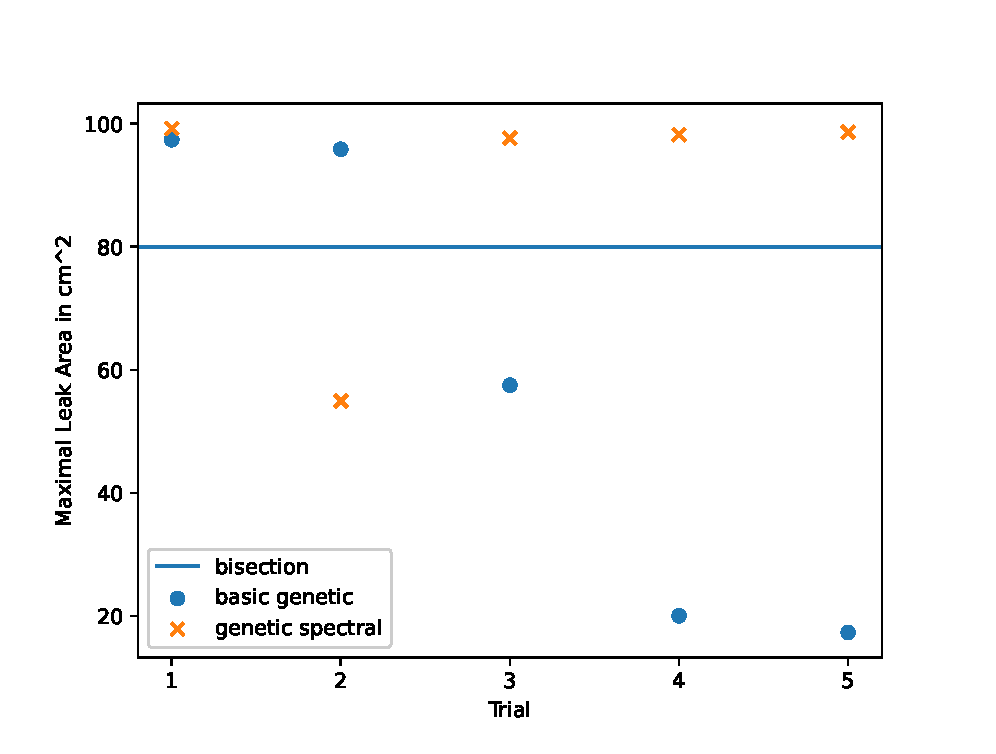
\includegraphics[width=\textwidth,height=0.3\textheight,keepaspectratio=true]{Figures/algorithm_comparison_ltown.eps}
\caption{Comparison of the three algorithmic approaches. }
\label{fig:luca_ftw}
\end{figure}

